
\documentclass[twocolumn]{article}
\usepackage{mathpazo}
\usepackage{microtype}
\usepackage{times}
\usepackage{titlesec} % 1
%\usepackage{sectsty} % "제 1 절" ...

 %%%%%%%%%%%%%%%%%%%%%%%%%%%%%%%%%%%%%%%%%%%%%%%%%%%%%%%%%%%%%%%%%%%%%%%%%%%%%
 %                              My Commands
\newcommand{\bi}{\begin{itemize}}
\newcommand{\ei}{\end{itemize}}
\newcommand{\be}{\begin{enumerate}}
\newcommand{\ee}{\end{enumerate}}
\newcommand{\ii}{\item}
\newtheorem{Def}{Definition}
\newtheorem{Lem}{Lemma}
\usepackage{algorithm}
\usepackage{algorithmicx}
\usepackage{algpseudocode}

\usepackage{graphicx}
\graphicspath{%
        {converted_graphics/}
        {./images/}
}
\usepackage{hyperref}
\usepackage{listings}

%\usepackage[hangul,nonfrench,finemath]{kotex}
    
\setlength\textwidth{7in} 
\setlength\textheight{9.5in} 
\setlength\oddsidemargin{-0.25in} 
\setlength\topmargin{-0.25in} 
\setlength\headheight{0in} 
\setlength\headsep{0in} 
\setlength\columnsep{9pt}
\sloppy 
 
\begin{document}

\title{
\vspace{-0.5in}\rule{\textwidth}{2pt}
\begin{tabular}{ll}\begin{minipage}{4.75in}\vspace{6px}
\noindent\large {\it KIWI Project}@Data Management Research Section\\
\vspace{-12px}\\
\noindent\LARGE ETRI\qquad  \large Technical Report 14ZS1410-TR-64
\end{minipage}&\begin{minipage}{2in}\vspace{6px}\small
218 Gajeong-ro, Yuseong-gu\\
Daejeon, 305-700, South Korea\\
http:/$\!$/www.etri.re.kr/\\
http:/$\!$/sungsoo.github.com/\quad 
\end{minipage}\end{tabular}
\rule{\textwidth}{2pt}\vspace{0.25in}
\LARGE \bf Analysis of the Apache Tez Design
}

\date{}

\author{
{\bf Sung-Soo Kim}\\
\it{sungsoo@etri.re.kr}
}

\maketitle

\begin{abstract}
{\small
MapReduce has served us well. For years it has been the processing
engine for Hadoop and has been the backbone upon which a huge amount of
value has been created. While it is here to stay, new paradigms are also
needed in order to enable Hadoop to serve an even greater number of
usage patterns. A key and emerging example is the need for
\emph{interactive query}, which today is challenged by the
\emph{batch-oriented nature} of MapReduce. A key step to enabling this
new world was \emph{Apache YARN} and today the community proposes the
next step\ldots{} \emph{Tez}}
\end{abstract}

\section{Introduction}
Apache Hadoop 2.0 (aka \textbf{YARN}) continues to make its way through the open source community process at the Apache Software Foundation and is getting closer to being declared “ready” from a community development perspective.  YARN on its own provides many benefits over Hadoop 1.x and its Map-Reduce job execution engine:

\bi
\ii Concurrent cluster applications via \textit{multiple independent AppMasters}
\ii Reduced job \textit{startup overheads}
\ii \textit{Pluggable} scheduling policy framework
\ii Improved \textit{security} framework
\ei

The support for third party AppMasters is the crucial aspect to flexibility in YARN.  It permits new job runtimes in addition to classical map-reduce, whilst still keeping M/R available and allowing both the old and new to co-exist on a single cluster.  \textbf{Apache Tez} is one such job runtime that provides richer capabilities than traditional map-reduce \cite{hortonworks}.  The motivation is to provide a better runtime for scenarios such as relational-querying that do not have a strong affinity for the map-reduce primitive.   This need arises because the Map-Reduce primitive mandates a very particular shape to every job and although this mandatory shape is very general and can be used to implement essentially any batch-oriented data processing job, it conflates too many details and provides too little flexibility.

The common behavior of a Map-Reduce job under Hadoop 1.x is as follows.

\be
\ii Client-side determination of input pieces
\ii Job startup
\ii Map phase, with optional in-process combiner \\
Each mapper reads input from durable storage
\ii Hash partition with local per-bucket sort.
\ii Data movement via framework initiated by reduce-side pull mechanism
\ii Ordered merge
\ii Reduce phase
\ii Write to durable storage
\ee

The map-reduce primitive has proved to be very useful as the basis of a reliable cluster computation runtime and it is well suited to data processing tasks that involve a small number of jobs that benefit from the standard behavior.  However, algorithms that require \textit{many iterations} suffer from the \textit{high overheads of job startup} and from frequent reads and writes to durable storage.  \textit{Relation query languages} such as Hive suffer from those issues and from the need to massage multiple datasets into homogeneous inputs as a M/R job can only consume one physical dataset (excluding support for side-data channels such as \textit{distributed cache}).  

\subsection{What is Tez?}

\textbf{Tez} -- Hindi for ``\emph{speed}'' provides a general-purpose, highly customizable
framework that creates simplifies data-processing tasks across both
small scale (low-latency) and large-scale (high throughput) workloads in
Hadoop \cite{Saha:2013-01}. It generalizes the MapReduce paradigm to a more powerful
framework by providing the ability to execute a complex \textbf{DAG}
(\emph{directed acyclic graph}) of tasks for a single job so that
projects in the Apache Hadoop ecosystem such as Apache Hive, Apache Pig
and Cascading can meet requirements for human-interactive response times
and extreme throughput at petabyte scale (clearly MapReduce has been a
key driver in achieving this).

\subsection{What Tez Does}

Tez is the logical next step for Apache Hadoop after \textbf{Apache
Hadoop YARN}. With YARN the community generalized Hadoop MapReduce to
provide a \emph{general-purpose resource management framework} wherein
MapReduce became merely one of the applications that could process data
in a Hadoop cluster. Tez provides a more general data-processing
application to the benefit of the entire ecosystem.

Tez will speed Pig and Hive workloads by an order of magnitude. By
eliminating unnecessary tasks, synchronization barriers, and reads from
and write to HDFS, Tez speeds up data processing across both
small-scale, low-latency and large-scale, high-throughput workloads.

\begin{figure}[htb]
        \centering
        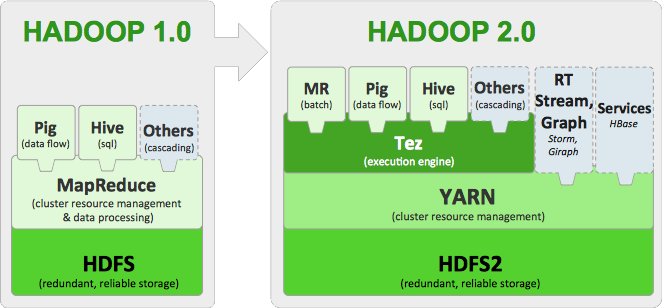
\includegraphics[width=0.48\textwidth]{hadoopstack}
        \caption{Hadoop 1.0 vs. Hadoop 2.0}
        \label{fig01}
\end{figure}

With the emergence of Apache Hadoop YARN as the basis of next generation
data-processing architectures, there is a strong need for an application
which can execute a complex DAG of tasks which can then be shared by
Apache Pig, Apache Hive, Cascading and others as shown in Figure \ref{fig01}. The constrained DAG
expressible in MapReduce (one set of maps followed by one set of
reduces) often results in multiple MapReduce jobs which harm latency for
short queries (overhead of launching multiple jobs) and throughput for
large-scale queries (too much overhead for materializing intermediate
job outputs to the filesystem). With Tez, we introduce a more expressive
DAG of tasks, within a single application or job, that is better aligned
with the required processing task -- thus, for e.g., any \emph{given SQL
query can be expressed as a single job} using Tez.

Figure \ref{fig02} illustrates the advantages provided by Tez for complex
SQL queries in Apache Hive or complex Apache Pig scripts.

\begin{figure}[htb]
        \centering
        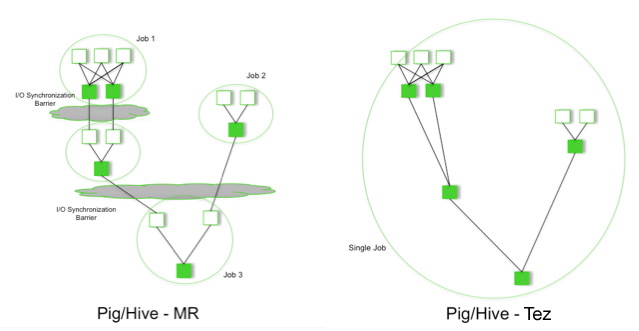
\includegraphics[width=0.48\textwidth]{pighivetez.png}
        \caption{General example of a Map-Reduce execution plan compared to DAG execution plan}
        \label{fig02}
\end{figure}

Tez is critical to the
\href{http://hortonworks.com/blog/100x-faster-hive}{\textbf{Stinger
Initiative}} and goes a long way in helping Hive support both
interactive queries and batch queries. Tez provides a single underlying
framework to support both latency and throughput sensitive applications,
there-by obviating the need for multiple frameworks and systems to be
installed, maintained and supported, a \emph{key advantage to
enterprises looking to rationalize their data architectures}.

Essentially, Tez is the logical next step for Apache Hadoop after Apache
Hadoop YARN. With YARN the community generalized Hadoop MapReduce to
provide a
\href{http://hortonworks.com/blog/introducing-apache-hadoop-yarn/}{general-purpose
resource management framework}(YARN) where-in MapReduce became merely
\emph{one of the applications} that could process data in your Hadoop
cluster. With Tez, we build on YARN and our experience with the
MapReduce to provide a more general data-processing application to the
benefit of the entire ecosystem i.e. Apache Hive, Apache Pig etc.

\subsection{Motivation}

\emph{Distributed data processing} is the core application that Apache
Hadoop is built around \cite{FOWLER:2013}.  Storing and analyzing \emph{large volumes} and
\emph{variety} of data efficiently has been the cornerstone use case
that has driven large scale adoption of Hadoop, and has resulted in
creating enormous value for the Hadoop adopters. Over the years, while
building and running data processing applications based on MapReduce, we
have understood a lot about the strengths and weaknesses of this
framework and how we would like to evolve the \emph{Hadoop data
processing framework} to meet the evolving needs of Hadoop users. As the
Hadoop compute platform moves into its next phase with \textbf{YARN}, it
has decoupled itself from MapReduce being the only application, and
opened the opportunity to create a new data processing framework to meet
the new challenges. Apache Tez aspires to live up to these lofty goals.

\section{Key Design Themes}

Higher-level data processing applications like Hive and Pig need an
\textit{execution framework} that can express their complex query logic in an
efficient manner and then execute it with \textit{high performance}. 
Apache Tez has been built around the following main design themes that solve these
key challenges in the Hadoop data processing domain.

\subsection{Ability to express, model and execute data processing logic}

Tez models data processing as a \emph{dataflow graph} with vertices in
the graph representing \emph{application logic} and edges representing
\emph{movement of data}. A rich dataflow definition API allows users to
express \emph{complex query logic} in an intuitive manner and it is a
natural fit for \emph{query plans} produced by higher-level declarative
applications like \textbf{Hive} and \textbf{Pig}. As an example, the
diagram shows how to model an \emph{ordered distributed sort} using
\textbf{range partitioning}. The \emph{Preprocessor} stage sends samples
to a \textbf{Sampler} that calculates sorted data ranges for each data
partition such that the work is \emph{uniformly distributed}. The ranges
are sent to \textbf{Partition} and \textbf{Aggregate} stages that read
their assigned ranges and perform the data \emph{scatter-gather}. This
dataflow pipeline can be expressed as a single Tez job that will run the
entire computation. Expanding this logical graph into a physical graph
of tasks and executing it is taken care of by Tez.

\begin{figure}[htb]
        \centering
        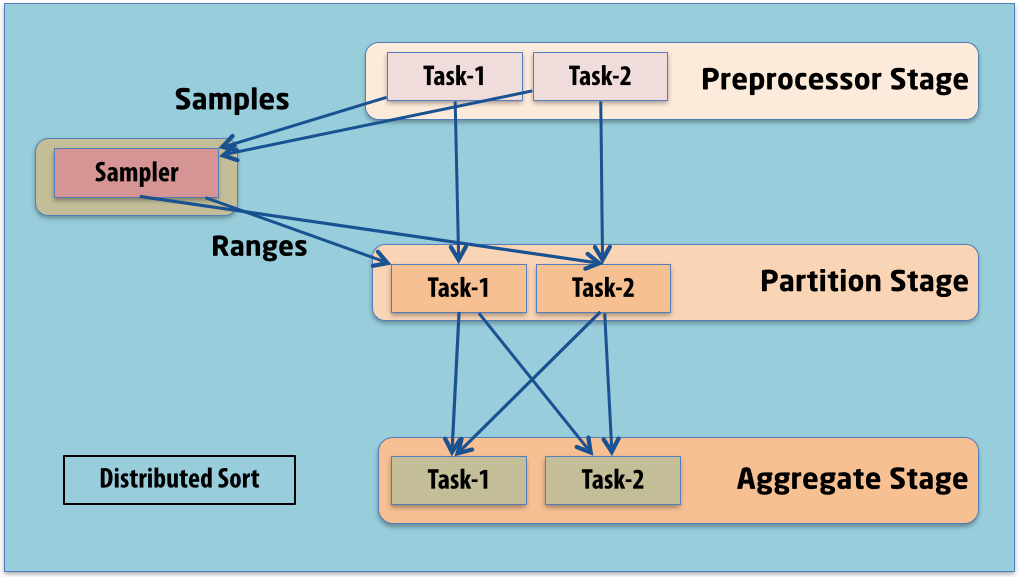
\includegraphics[width=0.48\textwidth]{tez1}
        \caption{DAG execution}
        \label{fig03}
\end{figure}

\subsection{Flexible Input-Processor-Output task model}

Tez models the user logic running in each vertex of the dataflow graph
as a composition of \textbf{Input}, \textbf{Processor} and
\textbf{Output} modules. Input \& Output determine the \emph{data
format} and how and where it is read/written. \emph{Processor} holds the
\emph{data transformation} logic. Tez does not impose any data format
and only requires that a combination of Input, Processor and Output must
be compatible with each other with respect to their formats when they
are composed to instantiate a \emph{vertex task}. Similarly, an Input
and Output pair connecting two tasks should be compatible with each
other. In the diagram, we can see how composing different Inputs,
Outputs and Processors can produce different tasks.

\begin{figure}[htb]
        \centering
        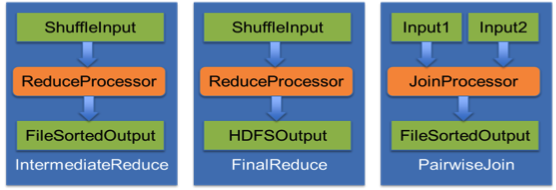
\includegraphics[width=0.48\textwidth]{tez2}
        \caption{DAG execution}
        \label{fig04}
\end{figure}

\subsection{Performance via Dynamic Graph Reconfiguration}

Distributed data processing is \emph{dynamic} by nature and it is
extremely difficult to statically determine \emph{optimal concurrency}
and \emph{data movement methods} a priori. More information is available
during runtime, like data samples and sizes, which may help optimize the
\emph{execution plan} further. We also recognize that Tez by itself
cannot always have the smarts to perform these \emph{dynamic
optimizations}. The design of Tez includes support for pluggable vertex
management modules to collect relevant information from tasks and change
the dataflow graph at runtime to optimize for performance and resource
usage. The diagram shows how Tez can determine an appropriate number of
reducers in a MapReduce like job by observing the actual data output
produced and the desired load per reduce task.

\begin{figure}[htb]
        \centering
        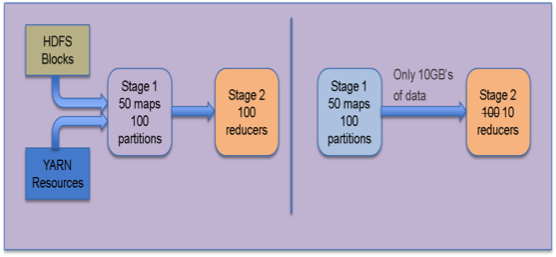
\includegraphics[width=0.48\textwidth]{tez3}
        \caption{Plan Reconfiguration at Runtime}
        \label{fig05}
\end{figure}

\subsection{Performance via Optimal Resource Management}

Resources acquisition in a \emph{distributed multi-tenant environment}
is based on cluster capacity, load and other quotas enforced by the
\emph{resource management framework} like \textbf{YARN}. Thus resource
available to the user may vary over time and over different executions
of the job. It becomes paramount to be able to efficiently use all
available resources to run a job as fast as possible during one instance
of execution and predictably over different instances of execution. The
Tez execution engine framework allows for efficient acquisition of
resources from YARN along with \emph{extensive reuse} of every component
in the pipeline such that no operation is duplicated unnecessarily.
These efficiencies are exposed to user logic, where possible, such that
users may also leverage this for \emph{efficient caching} and avoid
\emph{work duplication}. The diagram shows how Tez runs multiple
containers within the same YARN container host and how users can
leverage that to store their own objects that may be shared across
tasks.

\begin{figure}[htb]
        \centering
        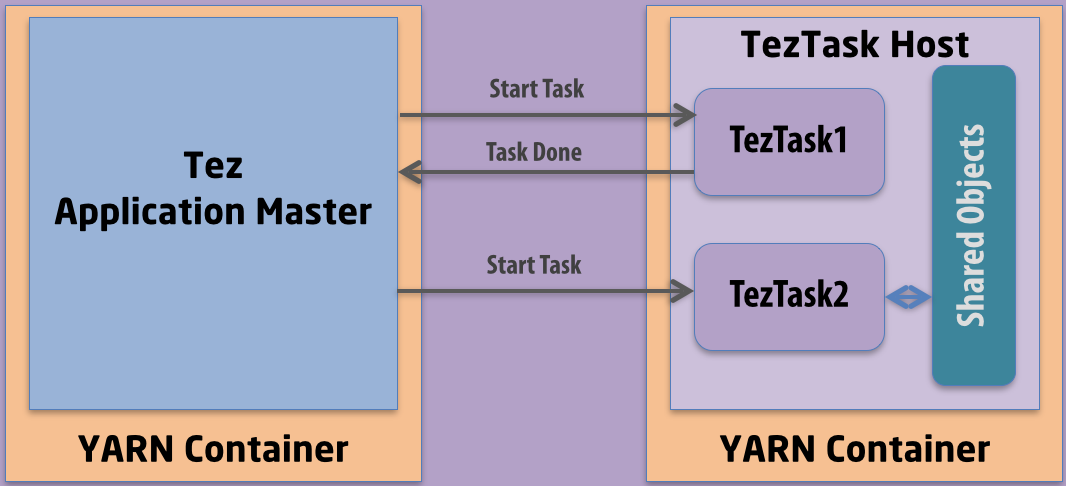
\includegraphics[width=0.48\textwidth]{tez4}
        \caption{Optimal Resource Management}
        \label{fig06}
\end{figure}


%We hope this brief overview about the philosophy and design of
%\textbf{Apache Tez} will throw some light on the aspirations of the
%project and how we hope to work with the Apache Hadoop community to
%bring them to life. \textbf{Apache Hive} and \textbf{Apache Pig}
%projects have already show deep interest in integrating with Tez.

%In the next posts in this series, we'll dive further into the
%\textbf{DAG execution} architecture, and look at MapReduce atop Tez
%along with the associated performance benefits of that model.


\section{Data Processing API in Apache Tez}
\subsection{Overview}

Apache Tez models data processing as a \emph{dataflow graph}, with the
\textbf{vertices} in the graph representing \emph{processing of data}
and \textbf{edges} representing \emph{movement of data} between the
processing. Thus \emph{user logic}, that analyses and modifies the data,
sits in the \textbf{vertices}. Edges determine the consumer of the data,
how the data is transferred and the \emph{dependency} between the
\emph{producer} and \emph{consumer} vertices. This model concisely
captures the \emph{logical definition of the computation}. When the Tez
job executes on the cluster, it expands this \emph{logical graph} into a
\emph{physical graph} by adding parallelism at the vertices to scale to
the data size being processed. Multiple tasks are created per logical
vertex to perform the computation in parallel.

\subsection{DAG Definition API}

More technically, the data processing is expressed in the form of a
\emph{directed acyclic graph} (\textbf{DAG}). The processing starts at
the root vertices of the DAG and continues down the \emph{directed
edges} till it reaches the leaf vertices. When all the vertices in the
DAG have completed then the data processing job is done. The graph does
not have cycles because the \emph{fault tolerance mechanism} used by Tez
is \textbf{re-execution} of failed tasks. When the input to a task is
lost then the producer task of the input is re-executed and so Tez needs
to be able to \emph{walk up} the graph edges to locate a non-failed task
from which to re-start the computation. \emph{Cycles} in the graph can
make this walk \emph{difficult} to perform. In some cases, cycles may be
handled by \emph{unrolling} them to create a DAG.

Tez defines a simple Java API to express a DAG of data processing \cite{Saha:2013-02}. 
The API has three components

\begin{itemize}
\item
  \textbf{DAG.} this defines the overall job. The user creates a DAG
  object for each data processing job.
\item
  \textbf{Vertex.} this defines the user logic and the resources \&
  environment needed to execute the user logic. The user creates a
  Vertex object for each step in the job and adds it to the DAG.
\item
  \textbf{Edge.} this defines the connection between producer and
  consumer vertices. The user creates an Edge object and connects the
  producer and consumer vertices using it.
\end{itemize}

\begin{figure}[htb]
        \centering
        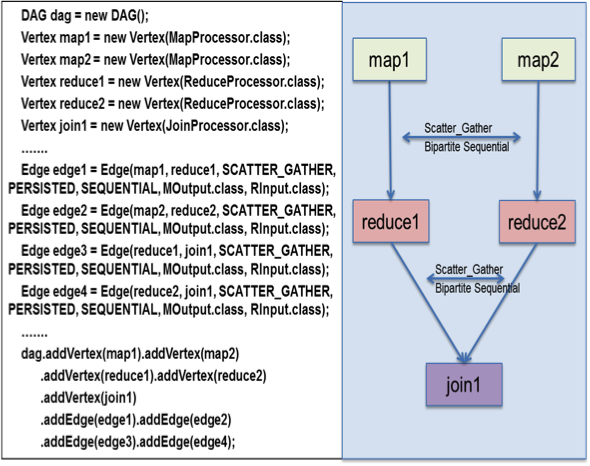
\includegraphics[width=0.48\textwidth]{tez11}
        \caption{DAG execution}
        \label{fig07}
\end{figure}

The diagram shows a \emph{dataflow graph} and its definition using the
DAG API (simplified). The job consists of 2 vertices performing a
``\textbf{Map}'' operation on 2 datasets. Their output is consumed by 2
vertices that do a ``\textbf{Reduce}'' operation. Their output is
brought together in the last vertex that does a ``\textbf{Join}''
operation.

Tez handles expanding this \emph{logical graph} at runtime to perform
the operations \emph{in parallel} using multiple tasks. The diagram
shows a runtime expansion in which the first M-R pair has a parallelism
of 2 while the second has a parallelism of 3. Both branches of
computation merge in the \textbf{Join operation} that has a parallelism
of 2. \emph{Edge properties} are at the heart of this runtime activity.

\begin{figure}[htb]
        \centering
        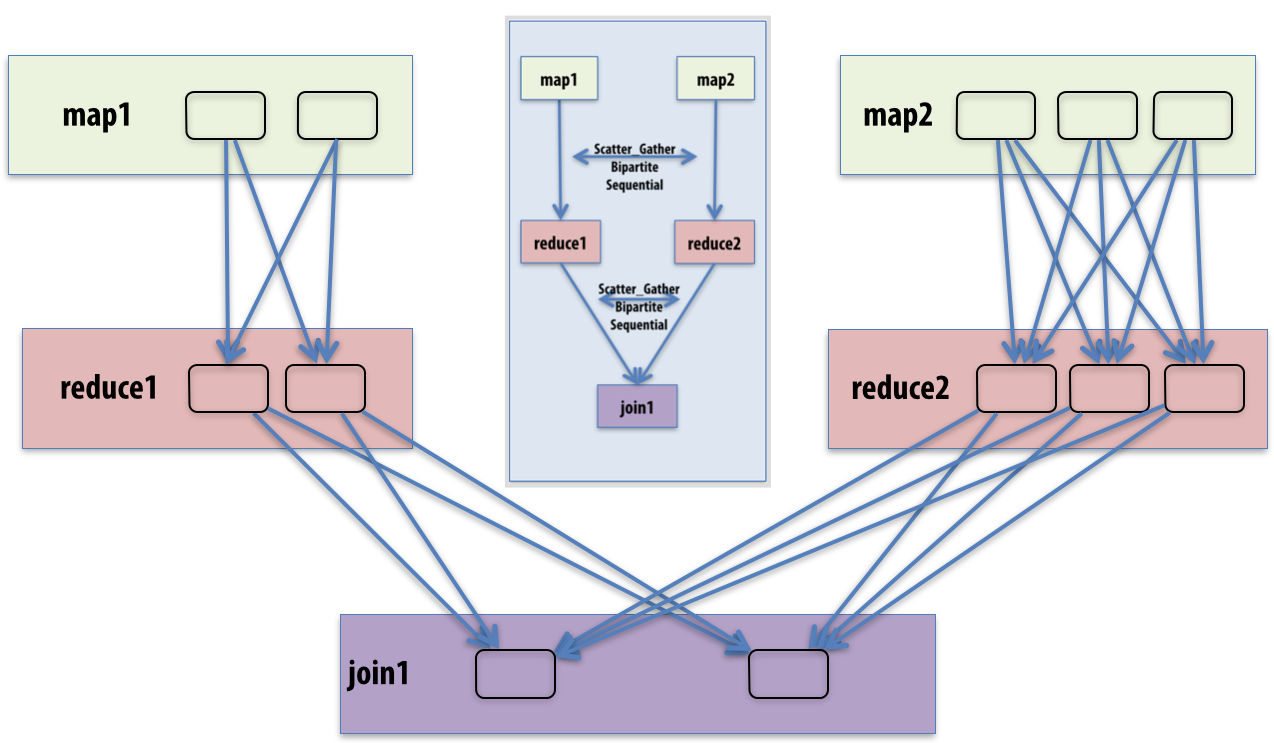
\includegraphics[width=0.48\textwidth]{tez21}
        \caption{DAG execution}
        \label{fig08}
\end{figure}

\subsection{Edge Properties}
The following edge properties enable Tez to instantiate the tasks,
configure their inputs and outputs, schedule them appropriately and help
\emph{route} the data between the tasks. The parallelism for each vertex
is determined based on \emph{user guidance}, \emph{data size} and
\emph{resources}.

\begin{itemize}
\item
  \textbf{Data movement.} Defines \emph{routing} of data between tasks
  \begin{itemize}
  \item
    \emph{One-To-One}: Data from the \emph{i}th producer task routes to
    the \emph{i}th consumer task.
  \item
    \emph{Broadcast}: Data from a producer task routes to \emph{all}
    consumer tasks.
  \item
    \emph{Scatter--Gather}: Producer tasks \emph{scatter} data into
    \emph{shards} and consumer tasks \emph{gather} the \emph{shards}.
    The \emph{i}th shard from all producer tasks routes to the
    \emph{i}th consumer task.
  \end{itemize}
\item
  \textbf{Scheduling.} Defines when a \emph{consumer} task is
  scheduled
  \begin{itemize}
  \item
    \emph{Sequential}: Consumer task may be scheduled after a
    \emph{producer task} completes.
  \item
    \emph{Concurrent}: Consumer task must be \emph{co-scheduled} with a
    producer task.
  \end{itemize}
\item
  \textbf{Data source.} Defines the \emph{lifetime}/\emph{reliability}
  of a task output
  \begin{itemize}
  \item
    \emph{Persisted}: Output will be available after the task exits.
    Output may be lost later on.
  \item
    \emph{Persisted-Reliable}: Output is reliably stored and will always
    be available
  \item
    \emph{Ephemeral}: Output is available only while the producer task
    is running
  \end{itemize}
\end{itemize}

\begin{figure}[htb]
        \centering
        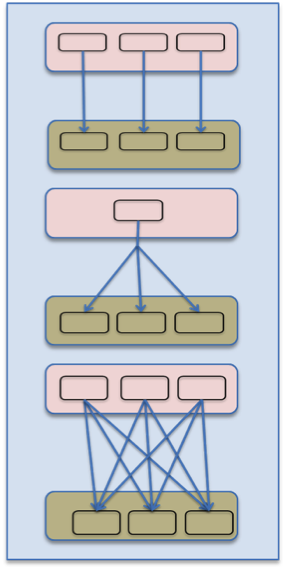
\includegraphics[width=0.2\textwidth]{tez31}
        \caption{DAG execution}
        \label{fig09}
\end{figure}

Some real life use cases will help in clarifying the edge properties.
\textbf{Mapreduce} would be expressed with the \emph{scatter-gather},
\emph{sequential} and \emph{persisted} edge properties. \textbf{Map
tasks} \emph{scatter} partitions and reduce tasks gather them.
\textbf{Reduce tasks} are \emph{scheduled} after the map tasks complete
and the map task outputs are written to local disk and hence available
after the map tasks have completed. When a vertex \emph{checkpoints} its
output into HDFS then its \emph{output edge} has a
\emph{persisted-reliable} property. If a producer vertex is
\emph{streaming data} directly to a consumer vertex then the edge
between them has \emph{ephemeral} and \emph{concurrent} properties. A
\emph{broadcast} property is used on a \emph{sampler vertex} that
produces a \textbf{global histogram} of data ranges for \emph{range
partitioning}.

We hope that the Tez dataflow definition API will be able to express a
broad spectrum of \emph{data processing topologies} and enable higher
level languages to elegantly transform their queries into Tez jobs.

\section{Runtime API in Apache Tez}
Apache Tez models data processing as a \emph{dataflow graph}, with the
\textbf{vertices} in the graph representing \emph{processing of data}
and \textbf{edges} representing \emph{movement of data} between the
processing \cite{Saha:2013-03}. Thus \emph{user logic}, that analyses and modifies the data,
sits in the \textbf{vertices}. Edges determine the consumer of the data,
how the data is transferred and the \emph{dependency} between the
\emph{producer} and \emph{consumer} vertices.

For users of \textbf{MapReduce} (\textbf{MR}), the most primitive
functionality that Tez can provide is an ability to run a \emph{chain of
Reduce stages} as compared to a \emph{single} Reduce stage in the
current MR implementation. Via the Task API, Tez can do this and much
more by facilitating execution of any form of processing logic that does
not need to be retrofitted into a Map or Reduce task and also by
supporting multiple options of data transfer between different vertices
that are not restricted to the \textbf{MapReduce} \emph{shuffle
transport mechanism}.

\subsection{The Building Blocks of Tez}

The Task API provides the building blocks for a user to plug-in their
logic to analyze and modify data into the vertex and augment this
processing logic with the necessary plugins to \emph{transfer} and
\emph{route} data between vertices.

Tez models the user logic running in each vertex as a composition of a
set of Inputs, a Processor and a set of Outputs.

\begin{itemize}

\item
  \textbf{Input:} An input represents a pipe through which a processor
  can accept input data from a \emph{data source} such as HDFS or the
  output generated by another vertex.
\item
  \textbf{Processor:} The entity responsible for \emph{consuming} one or
  more Inputs and \emph{producing} one or more Outputs.
\item
  \textbf{Output:} An output represents a pipe through which a processor
  can generate output data for another vertex to consume or to a
  \emph{data sink} such as HDFS.
\end{itemize}

Given that an edge in a DAG is a logical entity that represents a number
of physical connections between the tasks of 2 connected vertices, to
improve ease of programmability for a developer implementing a new
Processor, there are 2 kinds of Inputs and Outputs to either expose or
hide the level of complexity:

\begin{itemize}
\item
  \textbf{Logical:} A corresponding pair of a \emph{LogicalInput} and a
  \emph{LogicalOutput} represent the \emph{logical edge} between 2
  vertices. The implementation of Logical objects hides all the
  underlying physical connections and exposes a single view to the
  data.
\item
  \textbf{Physical:} The pair of Physical Input and Output represents
  the \emph{connection} between a task of the \emph{Source vertex} and a
  task of a \emph{Destination vertex}.
\end{itemize}

An example of the \emph{Reduce stage} within an MR job would be a
\textbf{Reduce Processor} that receives data from the maps via
\textbf{ShuffleInput} and generates output to HDFS. Likewise, an
intermediate Reduce stage in an \textbf{MRR chain} would be quite
similar to the final Reduce stage except for the difference in the
Output type.

\begin{figure}[htb]
        \centering
        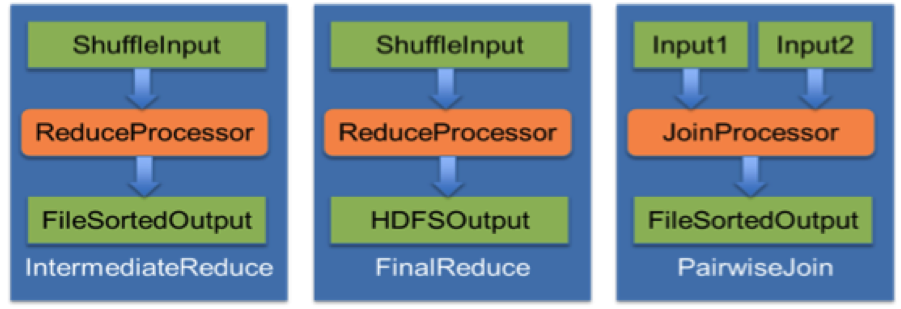
\includegraphics[width=0.48\textwidth]{tez12}
        \caption{DAG execution}
        \label{fig10}
\end{figure}


\subsection{Tez Runtime API}

\begin{figure}[htb]
        \centering
        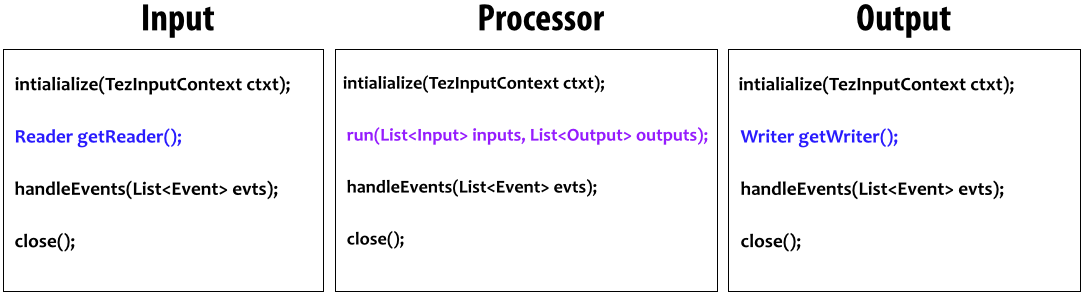
\includegraphics[width=0.48\textwidth]{tez32}
        \caption{DAG execution}
        \label{fig11}
\end{figure}


To implement a new Input, Processor or Output, a user to implement the
appropriate interfaces mentioned above. All objects are given a Context
object in their initialize functions. This context is the hook for these
objects to communicate to the \emph{Tez framework}. The Inputs and
Outputs are expected to provide implementations for their respective
Readers and Writers which are then used by the Processor to read/write
data. In a task, after the Tez framework has initialized all the
necessary Inputs, Outputs and the Processor, the Tez framework invokes
the Processor's run function and passes the appropriate handles to all
the Inputs and Outputs for that particular task.

Tez allows all inputs and outputs to be \emph{pluggable}. This requires
support for passing of information from the Output of a source vertex to
the Input of the destination vertex. For example, let us assume that the
Output of a source vertex writes all of its data to a \emph{key-value
store}. The Output would need to communicate the ``\textbf{key}'' to the
Input of the next stage so that the Input can retrieve the correct data
from the key-value store. To facilitate this, Tez uses \textbf{Events}.

\subsection{Events in Tez}

\emph{Events} in Tez are a way to pass information amongst different
components.

\begin{itemize}

\item
  The Tez framework uses Events to pass information of system events
  such as \emph{task failures} to the required components.
\item
  Inputs of a vertex can inform the framework of any failures
  encountered when trying to retrieve data from the source vertex's
  Output that in turn can be used by the framework to take failure
  recovery measures.
\item
  An Output can pass information of the location of the data, which it
  generates, to the Inputs of the destination vertex. An example of this
  is described in the Shuffle Event diagram which shows how the output
  of a Map stage informs the Shuffle Input of the Reduce stage of the
  location of its output via a Data Movement Event.
\end{itemize}

\begin{figure}[htb]
        \centering
        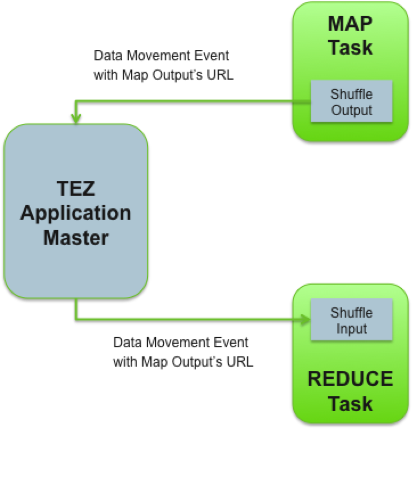
\includegraphics[width=0.4\textwidth]{tez22}
        \caption{DAG execution}
        \label{fig12}
\end{figure}


Another use of Events is to enable run-time changes to the DAG execution
plan. For example, based on the amount of the data being generated by a
Map stage, it may be more optimal to run less reduce tasks within the
following Reduce stage. Events generated by Outputs are routed to the
pluggable Vertex/Edge management modules, allowing them to make the
necessary decisions to modify some run-time parameters as needed.

\subsection{Available implementations of Inputs/Processors/Outputs}

The \emph{flexibility} of Tez allows anyone to implement their Inputs
and Outputs, whether they use \emph{blocking/non-blocking transport
protocols}, handle data in the form of raw bytes/records/key-value pairs
etc., and build Processors to handle these variety of Inputs and
Outputs.

There is already a small repository of various implementations of
Inputs/Outputs/Processors:

\begin{itemize}

\item
  \emph{MRInput} and \emph{MROutput}: Basic input and outputs to
  handle data to/from HDFS that are MapReduce compatible as they use
  MapReduce constructs such as InputFormat, RecordReader, OutputFormat
  and RecordWriter.
\item
  \emph{OnFileSortedOutput} and \emph{ShuffleMergedInput}: A pair of  key-value based Input and Output that use the local disk for all I/O
  and provide the same sort+merge functionality that is required for the
  ``shuffle'' edge between the Map and Reduce stages in a MapReduce job.
\item
  \emph{OnFileUnorderedKVOutput} and
  \emph{ShuffledUnorderedKVInput}: These are similar to the shuffle
  pair mentioned earlier except that the data is not sorted implicitly.
  This can be a big performance boost in various situations.
\item
  \emph{MapProcessor} and \emph{ReduceProcessor}: As the names
  suggest, these processors are available for anyone trying to run a
  MapReduce job on the Tez execution framework. They can be used to run
  an MRR chain too.
\end{itemize}

As the Hive and Pig projects adapt to use Tez, we hope this repository
will grow to house a common set of building blocks for use across the
different projects.

\section{Writing a Tez Input, Processor and Output}
\subsection{Tez Task}

Tez task is constituted of all the Inputs on its incoming edges, the
Processor configured for the Vertex, and all the Output(s) on it's
outgoing edge \cite{Saha:2013-04}.

The number of tasks for a vertex is equal to the parallelism set for
that vertex -- which is set at DAG construction time, or modified during
runtime via user plugins running in the AM.

\begin{figure}[htb]
        \centering
        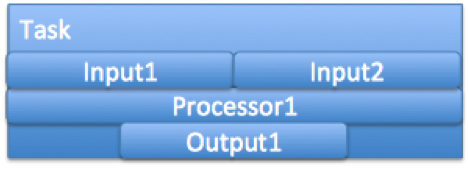
\includegraphics[width=0.48\textwidth]{tez01}
        \caption{tez01}
        \label{fig13}
\end{figure}


The diagram shows a single task. The vertex is configured to run
Processor1 -- has two incoming edges -- with the output of the edge
specified as Input1 and Input2 respectively, and has a single outgoing
edge -- with the input to this edge configured as Output1. There will be
n such Task instances created per Vertex -- depending on the
parallelism.

\subsection{Initialization of a Tez task}

The following steps are followed to initialize and run a Tez task.

The Tez framework will first construct instances of the specified
Input(s), Processor, Output(s) using a 0 argument constructor.

For a LogicalInput and a LogicalOutput -- the Tez framework will set the
number of physical connections using the respective setNumPhysicalInputs
and setNumPhysicalOutputs methods.

The Input(s), Processor and Output(s) will then be initialized via their
respective initialize methods. Configuration and context information is
made available to the Is/P/Os via this call. More information on the
Context classes is available in the JavaDoc for TezInputContext,
TezProcessorContext and TezOutputContext.

The Processor run method will be called with the initialized Inputs and
Outputs passed in as arguments (as a Map -- connected vertexName to
Input/Output).

Once the run method completes, the Input(s), Processor and Output(s)
will be closed, and the task is considered to be complete.

Notes for I/P/O writers:

Each Input / Processor / Output must provide a 0 argument constructor.
No assumptions should be made about the order in which the Inputs,
Processor and Outputs will be initialized, or closed. Assumptions should
also not be made about how the Initialization, Close and Processor run
will be invoked -- i.e. on the same thread or multiple threads.

\subsubsection{Common Interfaces to be implemented by
Input/Processor/Output}

List initialize(Tez*Context) -This is where I/P/O receive their
corresponding context objects. They can, optionally, return a list of
events. handleEvents(List events) -- Any events generated for the
specific I/P/O will be passed in via this interface. Inputs receive
DataMovementEvent(s) generated by corresponding Outputs on this
interface -- and will need to interpret them to retrieve data. At the
moment, this can be ignored for Outputs and Processors. List close() --
Any cleanup or final commits will typically be implemented in the close
method. This is generally a good place for Outputs to generate
DataMovementEvent(s). More on these events later.

\subsubsection{Providing User Information to an Input / Processor /
Output}

Information specified in the bytePayload associated with an
Input/Processor/Output is made available to the respective I/P/O via
their context objects.

Users provide this information as a byte array -- and can specify any
information that may be required at runtime by the I/P/O. This could
include configuration, execution plans for Hive/PIG, etc. As an example,
the current inputs use a Hadoop Configuration instance for backward
compatibility. Hive may choose to send it's vertex execution plan as
part of this field instead of using the distributed cache provided by
YARN.

Typically, Inputs and Outputs exist as a pair -- the Input knows how to
process DataMovementEvent(s) generated by the corresponding Output, and
how to interpret the data. This information will generally be encoded
into some form of configuration (specified via the userPayload) used by
the Output-Input pair, and should match. As an example -- the output Key
type configured on an Output should match the Input key type on the
corresponding Input.

\subsection{Writing a Tez LogicalOutput}

A LogicalOutput can be considered to have two main responsibilities --
1) dealing with the actual data provided by the Processor --
partitioning it for the `physical' edges, serializing it etc, and 2)
Providing information to Tez (in effect the subsequent Input) on where
this data is available.

\subsubsection{Processing the Data}

Depending on the connection pattern being used -- an Output will
generate data to a single `physical' edge or multiple `physical' edges.
A LogicalOutput is responsible for partitioning the data into these
`physical' edges.

It would typically work in conjunction with the configured downstream
Input to write data in a specific data format understood by the
downstream Input. This includes a serialization mechanism, compression
etc.

As an example: OnFileSortedOutput which is the Output used for a
MapReduce shuffle makes use of a Partitioner to partition the data into
n partitions (`physical' edges) -- where n corresponds to the number of
downstream tasks. It also sorts the data per partition, and writes it
out as Key-Value pairs using Hadoop serialization which is understood by
the downstream Input (ShuffledMergedInput in this case).

\subsubsection{Providing information on how the data is to be retrieved}

A LogicalOutput needs to send out information on how data is to be
retrieved by the corresponding downstream Input defined on an edge. This
is done by generating DataMovementEvent(s). These events are routed by
the AM, based on the connection pattern, to the relevant LogicalInputs.

These events can be sent at anytime by using the TezOutputContext with
which the Output was initialized. Alternately, they can be returned as
part of the initialize() or close() calls. More on DataMovementEvent(s)
further down.

Continuing with the OnFileSortedOutput example: This will generate one
event per partition -- the sourceIndex for each of these events will be
the partition number. This particular Output makes use of the MapReduce
ShuffleHandler, which requires downstream Inputs to pull data over HTTP.
The payload for these events contains the host name and port for the
http server, as well as an identifier which uniquely identifies the
specific task and Input instance running this output.

In case of OnFileSortedOutput -- these events are generated during the
close() call.

View OnFileSortedOutput.java

\subsubsection{Specific interface for a LogicalOutput}

setNumPhysicalOutputs(int) -- This is where a Logical Output is informed
about the number of physical outgoing edges for the output. Writer
getWriter() -- An implementation of the Writer interface, which can be
used by a Processor to write to this Output.

\subsection{Writing a Tez LogicalInput}

The main responsibilities of a Logical Input are 1) Obtaining the actual
data over the `physical' edges, and 2) Interpreting the data, and
providing a single `Logical' view of this data to the Processor.

\subsubsection{Obtaining the Data}

A LogicalInput will receive DataMovementEvent(s) generated by the
corresponding LogicalOutput which generated them. It needs to interpret
these events to get hold of the data. The number of DataMovementEvent(s)
a LogicalInput receives is typically equal to the number of physical
edges it is configured with, and is used as a termination condition.

As an example: ShuffledMergedInput (which is the Input on the
OnFileSortedOutput-ShuffledMergedInput O-I edge) would fetch data from
the ShuffleHandler by interpretting the host, port and identifier from
the DataMovementEvent(s) it receives.

\subsubsection{Providing a view of the data to the Processor}

A LogicalInput will typically expose the data to the Processor via a
Reader interface. This would involve interpreting the data, manipulating
it if required -- decompression, ser-de etc.

Continuing with the ShuffledMergedInput example: This input fetches all
the data -- one chunk per source task and partition -- each of which is
sorted. It then proceeds to merge the sorted chunks and makes the data
available to the Processor only after this step -- via a KeyValues
reader implementation.

View ShuffledMergedInput.java

View ShuffledUnorderedKVInput.java

\subsubsection{Specific interface for a LogicalInput}

setNumPhysicalInputs(int) -- This is where a LogicalInput is informed
about the number of physical incoming edges. Reader getReader() -- An
implementation of the Reader interface, which can be used by a Processor
to read from this Input

\subsection{Writing a Tez LogicalIOProcessor}

A logical processor receives configured LogicalInput(s) and
LogicalOutput(s). It is responsible for reading source data from the
Input(s), processing it, and writing data out to the configured
Output(s).

A processor is aware of which vertex (vertex-name) a specific Input is
from. Similarly, it is aware of the output vertex (via the vertex-name)
associated with a specific Output. It would typically validate the Input
and Output types, process the Inputs based on the source vertex and
generate output for the various destination vertices.

As an example: The MapProcessor validates that it is configured with
only a single Input of type MRInput -- since that is the only input it
knows how to work with. It also validates the Output to be an
OnFileSortedOutput or a MROutput. It then proceeds to obtain a KeyValue
reader from the MRInput, and KeyValueWriter from the OnFileSortedOutput
or MROutput. The KeyvalueReader instance is used to walk all they keys
in the input -- on which the user configured map function is called,
with a MapReduce output collector backed by the KeyValue writer
instance.

\subsubsection{Specific interface for a LogicalIOProcessor}

run(Map inputs, Map outputs) -- This is where a processor should
implement it's compute logic. It receives initialized Input(s) and
Output(s) along with the vertex names to which the Input(s) and
Output(s) are connected.

\subsection{Data Movement Event}

A DataMovementEvent is used to communicate between Outputs and Inputs to
specify location information. A byte payload field is available for this
-- the contents of which should be understood by the communicating
Outputs and Inputs. This byte payload could be interpreted by
user-plugins running within the AM to modify the DAG (Auto
reduce-parallelism as an example).

DataMovementEvent(s) are typically generated per physical edge between
the Output and Input. The event generator needs to set the sourceIndex
on the event being generated -- and this matches the physical
Output/Input that generated the event. Based on the ConnectionPattern
specified for the DAG -- Tez sets the targetIndex, so that the event
receiver knows which physical Input/Output the event is meant for. An
example of data movement events generated by a ScatterGather connection
pattern (Shuffle) follows, with values specified for the source and
target Index.

\begin{figure}[htb]
        \centering
        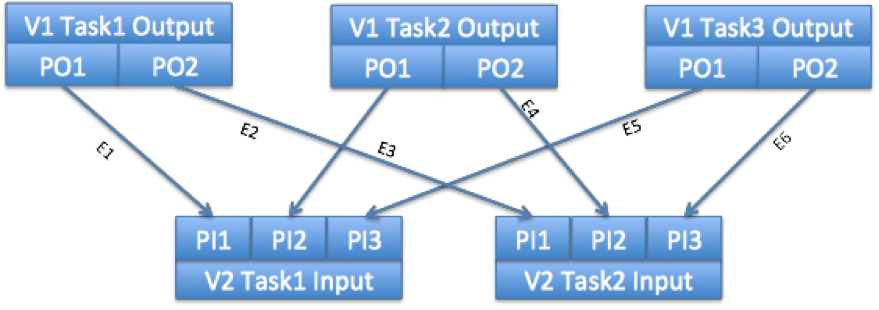
\includegraphics[width=0.48\textwidth]{tez02}
        \caption{tez01}
        \label{fig14}
\end{figure}

In this case the Input has 3 tasks, and the output has 2 tasks. Each
input generates 1 partition (physical output) for the downstream tasks,
and each downstream task consumes the same partition from each of the
upstream tasks.

Vertex1, Task1 will generate two DataMovementEvents -- E1 and E2. E1,
sourceIndex = 0 (since it is generated by the 1st physical output) E2,
sourceIndex = 1 (since it is generated by the 2nd physical output)

Similarly Vertex1, Task2 and Task3 will generate two data movement
events each. E3 and E5, sourceIndex=0 E4 and E6, sourceIndex=1

Based on the ScatterGather ConnectionPattern, the AM will rout the
events to respective tasks. E1, E3, E5 with sourceIndex 1 will be sent
to Vertex2, Task1 E2, E4, E6 with sourceIndex 2 will be sent to Vertex2,
Task2

The destination will see the following targetIndex (based on the
physical edges between the tasks (arrows)) E1, targetIndex=0 -- first
physical input to V2, Task1 E3, targetIndex=1 -- second physical input
to V2, Task1 E5, targetIndex=5 -- third physical input to V2, Task1
Similarly, E2, E4, E6 will have target indices 0,1 and 2 respectively --
i.e. first, second and third physical input to V2 Task2.

DataMovement events generated by an Input are routed to the
corresponding upstream Input defined on the edge. Similarly data
movement events generated by an Output are routed to the corresponding
downstream Input defined on the edge.

If the Output is one of the Leaf Outputs for a DAG -- it will typically
not generate any events.

\subsection{Error Handling}

Reporting errors from an Input/Processor/Output Fatal Errors -- fatal
errors can be reported to Tez via the fatalError method available on the
context instances, with which the I/P/O was initialized. Alternately,
throwing an Exception from the initialize, close or run methods are
considered to be fatal. Fatal errors cause the current running task to
be killed. Actionable Non Fatal Errors -- Inputs can report the failure
to obtain data from a specific Physical connection by sending an
InputReaderErrorEvent via the InputContext. Depending on the Edge
configuration, this may trigger a retry of the previous stage task which
generated this data. Errors reported to an Input If the AM determines
that data generated by a previous task is no longer available, Inputs
which require this data are informed via an InputFailedEvent. The
sourceIndex, targetIndex and attemptNumber information on this event
would correspond to the DataMovementEvent event with the same values.
The Input will typically handle this event by not attempting to obtain
data based on the specific DataMovement event, and would wait for an
updated DataMovementEvent for the same data.

Notes on Reader and Writer Tez does not enforce any interface on the
Reader and Writer to stay data format agnostic. Specific Writers and
Readers can be implemented for Key-Value, Record or other data formats.
A KeyValue and KeyValues Reader/Writer interface and implementation,
based on Hadoop serialization, is used by the Shuffle Input/Output
provided by the Tez Runtime library.

\section{Apache Tez Dynamic Graph Reconfiguration}
\subsection{Case Study: Automatic Reduce Parallelism}

\subsubsection{Motivation}

\emph{Distributed data processing} is dynamic by nature and it is
extremely difficult to statically determine \emph{optimal concurrency}
and \emph{data movement methods} a priori. More information is available
during runtime, like \emph{data samples and sizes}, which may help
optimize the execution plan further. We also recognize that Tez by
itself cannot always have the smarts to perform these \emph{dynamic
optimizations}. The design of Tez includes support for \emph{pluggable
vertex management} modules to collect relevant information from tasks
and change the \emph{dataflow graph} at runtime to optimize for
\textbf{performance} and \textbf{resource usage} \cite{Saha:2013-05}. The diagram shows how
we can determine an appropriate number of reducers in a MapReduce like
job by observing the actual data output produced and the \emph{desired
load} per reduce task.

\begin{figure}[htb]
        \centering
        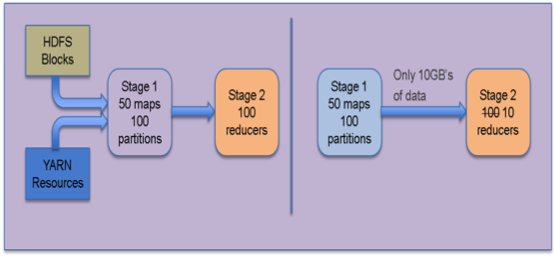
\includegraphics[width=0.48\textwidth]{dtez11}
        \caption{tez01}
        \label{fig15}
\end{figure}

\subsubsection{Performance \& Efficiency via Dynamic Graph
Reconfiguration}

Tez envisions running computation by the most \emph{resource efficient}
and \emph{high-performance} means possible given the runtime conditions
in the cluster and the results of the previous steps of the computation.
This functionality is constructed using a couple of basic building
blocks

\begin{itemize}
\item
  \textbf{Pluggable Vertex Management Modules}: The control flow
  architecture of Tez incorporates a \emph{per-vertex pluggable module}
  for user logic that deeply understands the data and computation. The
  vertex state machine invokes this user module at significant
  transitions of the state machine such as vertex start, source task
  completion etc. At these points the user logic can examine the runtime
  state and provide hints to the main Tez execution engine on attributes
  like vertex task parallelism.
\item
  \textbf{Event Flow Architecture}: Tez defines a set of events by which
  different components like vertices, tasks etc. can pass information to
  each other. These events are routed from source to destination
  components based on a \emph{well-defined routing logic} in the Tez
  control plane. One such event is the \textbf{VertexManager} event that
  can be used to send any kind of user-defined payload to the
  VertexManager of a given vertex.
\end{itemize}

\subsection{Case Study: Reduce task parallelism and Reduce Slow-start}

Determining the correct number of reduce tasks has been a long standing
issue for Map Reduce jobs. The output produced by the map tasks is not
known a priori and thus determining that number before job execution is
hard. This becomes even more difficult when there are several stages of
computation and the reduce parallelism needs to be determined for each
stage. We take that as a case study to demonstrate the graph
reconfiguration capabilities of Tez.

\paragraph{Reduce Task Parallelism:}

Tez has a \textbf{ShuffleVertexManager} that understands the semantics
of \emph{hash based partitioning} performed over a \emph{shuffle
transport layer} that is used in MapReduce. Tez defines a
\textbf{VertexManager} event that can be used to send an arbitrary user
payload to the vertex manager of a given vertex. The \emph{partitioning
tasks} (say the \textbf{Map tasks}) use this event to send
\emph{statistics} such as the size of the output partitions produced to
the \textbf{ShuffleVertexManager} for the reduce vertex. The manager
receives these events and tries to model the final output statistics
that would be produced by the all the tasks. It can then advise the
\emph{vertex state machine} of the Reduce vertex to decrease the
parallelism of the vertex if needed. The idea being to first
\emph{over-partition} and then determine the correct number at runtime.
The \emph{vertex controller} can cancel extra tasks and proceed as
usual.

\paragraph{Reduce Slow-start/Pre-launch:}

Slow-start is a MapReduce feature where-in the reduce tasks are launched
before all the map tasks complete. The hypothesis being that reduce
tasks can start fetching the completed map outputs while the remaining
map tasks complete. Determining when to pre-launch the reduce tasks is
tricky because it depends on output data produced by the map tasks. It
would be inefficient to run reduce tasks so early that they finish
fetching the data and sit idle while the remaining maps are still
running. In Tez, the \emph{slow-start logic} is embedded in the
\textbf{ShuffleVertexManager}. The vertex state controller informs the
manager whenever a \emph{source task} (here the \textbf{Map task})
completes. The manager uses this information to determine when to
\emph{pre-launch} the reduce tasks and how many to pre-launch. It then
advises the vertex controller.

Its easy to see how the above can be extended to determine the correct
parallelism for \emph{range-partitioning} scenarios. The data samples
could be sent via the \textbf{VertexManager} events to the vertex
manager that can create the \emph{key-range histogram} and determine the
correct number of partitions. It can then assign the appropriate
key-ranges to each partition. Thus, in Tez, this operation could be
achieved without the overhead of a separate sampling job.

\section{Re-Using Containers in Apache Tez}
\subsection{Motivation}

Tez follows the traditional Hadoop model of \emph{dividing a job into
individual tasks}, all of which are run as processes via \textbf{YARN},
on the users' behalf -- for \emph{isolation}, among other reasons. This
model comes with inherent costs -- some of which are listed below.

\begin{itemize}

\item
  Process \emph{startup} and \emph{initialization} cost, especially when
  running a Java process is fairly high. For short running tasks, this
  initialization cost ends up being a significant fraction of the actual
  task runtime. \emph{Re-using containers} can significantly reduce this
  cost.

\item
  Stragglers have typically been another problem for jobs -- where
  \emph{a job runtime is limited by the slowest running task}. With
  reduced static costs per tasks -- it becomes possible to run more
  tasks, each with a smaller work-unit. This reduces the runtime of
  stragglers (\emph{smaller work-unit}), while allowing faster tasks to
  process additional work-units which can \emph{overlap} with the
  stragglers.\\
\item
  \emph{Re-using containers} has the additional advantage of not needing
  to allocate each container via the \textbf{YARN ResourceManager (RM)} \cite{Saha:2013-06}.
\end{itemize}

Other than helping solve some of the existing concerns, re-using
containers provide additional opportunities for optimization where data
can be \emph{shared} between tasks.

\subsection{Consideration for Re-Using Containers}

\subsubsection{Compatibility of containers}

Each vertex in Tez specifies parameters, which are used when launching
containers. These include the requested resources (memory, CPU etc),
\textbf{YARN LocalResources}, the environment, and the command line
options for tasks belonging to this \textbf{Vertex}. When a container is
first launched, it is launched for a specific task and uses the
parameters specified for the \emph{task} (or \emph{vertex}) -- this then
becomes the container's signature. An already running container is
considered to be compatible for another task when the running
container's signature is a superset of what the task requires.

\subsubsection{Scheduling}

Initially, when no containers are available, the Tez AM will request
containers from the RM with location information specified, and rely on
YARN's scheduler for locality-aware assignments. However, for containers
which are being considered for re-use, the scheduling smarts offered by
YARN are no longer available.

The \textbf{Tez scheduler} works with several parameters to take
decisions on \emph{task assignments} -- \emph{task-locality
requirements}, \emph{compatibility of containers} as described above,
total available resources on the cluster, and the priority of pending
task requests.

When a task completes, and the container running the task becomes
available for re-use -- a task may not be assigned to it immediately --
as tasks may not exist, for which the data is local to the container's
node. The Tez scheduler first makes an attempt to find a task for which
the data would be \emph{local} for the container. If no such task
exists, the scheduler holds on to the container for a specific time,
before actually allocating any \emph{pending tasks} to this container.
The expectation here, is that more tasks will complete -- which gives
additional opportunities for scheduling tasks on nodes which are close
to the data. Going forward, \emph{non-local containers} may be used in a
speculative manner.

\emph{Priority} of pending tasks (across different vertices),
compatibility and cluster resources are considered to ensure that tasks
which are deemed to be of higher priority (either due to a
must-run-before relationship, failure, or due to specific scheduling
policies) have an available container.

In the future, \emph{affinity} will become part of the \emph{scheduling
decision}. This could be dictated by common resources shared between
tasks, which need only be loaded by the first task running in a
container, or by the data generated by the first task, which can then
directly be processed by subsequent tasks, without needing to
move/serialize the data -- especially in the case of \textbf{One-to-One
edges}.

\subsection{Beyond simple JVM Re-Use}

\subsubsection{Cluster Dependent Work Allocation}

At the moment, the number of tasks for a vertex, and their corresponding
`\textbf{work-units}' are determined up front. Going forward, this is
likely to change to a model, where a certain number of tasks are setup
up front based on cluster resources, but \emph{work-units} for these
tasks are determined at runtime. This allows additional optimizations
where tasks which complete early are given additional work, and also
allows for better \emph{locality-based assignment} of work.

\subsubsection{Object Registry}

Each Tez JVM (or \emph{container}) contains an \emph{object cache},
which can be used to \emph{share data} between different tasks running
within the same container. This is a simple \textbf{Key-Object store},
with different levels of \emph{visibility/retention}. Objects can be
cached for use within tasks belonging to the same Vertex, for all tasks
within a \textbf{DAG}, and for tasks running across a \textbf{Tez
Session} (more on Sessions in a subsequent post). The resources being
cached may, in the future, be made available as a hint to the Tez
Scheduler for affinity based \emph{scheduling}.

\subsubsection{Examples of usage:}

\begin{figure}[htb]
        \centering
        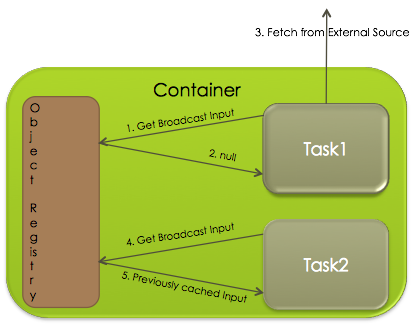
\includegraphics[width=0.48\textwidth]{tez121}
        \caption{tez01}
        \label{fig16}
\end{figure}

1) \textbf{Hive} makes use of this \emph{object registry} to cache data
for \textbf{Broadcast Joins}, which is fetched and computed once by the
first task, and used directly by remaining tasks which run in the same
JVM.

2) The sort buffer used by \emph{OnFileSortedOutput} can be cached,
and re-used across tasks.

\section{Tez Sessions}
\subsection{Introduction}

Most relational databases have had a notion of sessions for quite some
time. A database session can be considered to represent a connection
between a user/application and the database or in more general terms, an
instance of usage of a database. A session can encompass multiple
queries and/or transactions. It can leverage common services, for
example, caching, to provide some level of performance optimizations.

A Tez session, currently, maps to one instance of a Tez Application
Master (AM). For folks who are familiar with YARN and MapReduce, you
would know that for each MapReduce job, a corresponding MapReduce
Application Master is launched. In Tez, using a Session, a user can can
start a single Tez Session and then can submit DAGs to this Session AM
serially without incurring the overhead of launching new AMs for each
DAG.

\subsection{Motivation for Tez Sessions}

As mentioned earlier, the main proponents for Tez are Apache projects
such as Hive and Pig. Consider a Pig script, the amount of work
programmed into a script may not be doable within a single Tez DAG. Or
let us take a common data analytics use-case in Hive where a user uses a
Hive Shell for data drill-down (for example, multiple queries over a
common data-set). There are other more general use-cases such as users
of Hive connecting to the Hive Server and submitting queries over the
established connection or using the Hive shell to execute a script
containing one or more queries.

All of the above can leverage Tez Sessions \cite{Saha:2013-07}.

\begin{figure}[htb]
        \centering
        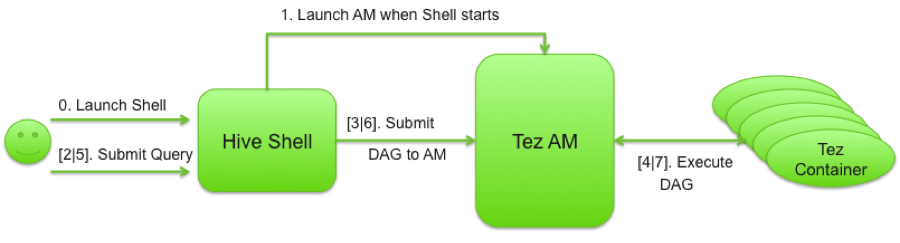
\includegraphics[width=0.48\textwidth]{sessions-tez1}
        \caption{tez01}
        \label{fig17}
\end{figure}

\subsection{Using Tez Sessions}

Using a Tez Session is quite simple:

\begin{enumerate}

\item
  Firstly, instantiate a \emph{TezSession} object with the required
  configuration using \emph{TezSessionConfiguration}.
\item
  Invoke \emph{TezSession::start()}
\item
  Wait for the TezSession to reach a ready state to accept DAGs by using
  the \emph{TezSession::getSessionStatus()} api (this step is
  optional)
\item
  Submit a DAG to the Session using
  \emph{TezSession::submitDAG(DAG dag)}
\item
  Monitor the DAG's status using the \emph{DAGClient} instance
  obtained in step (4).
\item
  Once the DAG has completed, repeat step (4) and step (5) for
  subsequent DAGs.
\item
  Shutdown the Session once all work is done via
  \emph{TezSession::stop()}.
\end{enumerate}

There are some things to keep in mind when using a Tez Session:

\begin{itemize}

\item
  A \textbf{Tez Session} maps to a single \textbf{Application Master}
  and therefore, all resources required by any user-logic (in any
  subsequent DAG) running within the \textbf{ApplicationMaster} should
  be available when the \textbf{AM} is launched.

  \begin{itemize}
  
  \item
    This mostly pertains to code related to the
    \textbf{VertexOutputCommitter} and any user-logic in the
    \textbf{Vertex} \emph{scheduling} and \emph{management} layers.
  \item
    User-logic run in tasks is not governed by the above restriction.
  \end{itemize}
\item
  The resources (memory, CPU) of the \textbf{AM} are fixed so please
  keep this in mind when configuring the AM for use in a session. For
  example, memory requirements may be higher for a very large DAG.
\end{itemize}

\subsection{Performance Benefits of using Tez Sessions}

\textbf{Container Re-Use}. We know that \emph{re-use} of containers was
doable within a single DAG. In a Tez Session, containers are re-used
even across DAGs as long as the containers are compatible with the task
to be run on them. This vastly improves performance by not incurring the
overheads of launching containers for subsequent DAGs. Containers, when
not in use, are kept around for a \emph{configurable period} before
being released back to YARN's \textbf{ResourceManager}.

\textbf{Caching with the Session}. When running drill-down queries on
common datasets, smarting caching of meta-data and potentially even
caching of intermediate data or previous results can help improve
performance. \emph{Caching} could be done either within the \textbf{AM}
or within \emph{launched containers}. Such caching allows for more
\emph{fine-grained controls} with respect to caching policies. A
\emph{session-based cache} as compared to a global cache potentially
provides more predictable performance improvements.

\subsection{Example Usage of a Tez Session}

The Tez source code has a
\href{https://git-wip-us.apache.org/repos/asf?p=incubator-tez.git;a=blob_plain;f=tez-mapreduce-examples/src/main/java/org/apache/tez/mapreduce/examples/OrderedWordCount.java;hb=master}{simple
\textbf{OrderedWordCount} example}. This DAG is similar to the
\textbf{WordCount} example in \textbf{MapReduce} except that it also
orders the words based on their frequency of occurrence in the dataset.
The DAG is an \textbf{MRR chain} i.e. a \emph{3-vertex linear chain} of
\textbf{Map-Reduce-Reduce}.

To run the \textbf{OrderedWordCount} example to process different
data-sets via a single Tez Session, use:

{\tiny
\begin{verbatim}
hadoop jar tez-mapreduce-examples.jar orderedwordcount 
-DUSE_TEZ_SESSION=true -DINTER_JOB_SLEEP_INTERVAL=0
/input1/ /output1/ /input2/ /output2/ /input3/ /output3/ /input4/ /output4/
\end{verbatim}
}

Below is a graph depicting the times seen when running \emph{multiple}
MRR DAGs on the same dataset (the dataset had 6 files to ensure multiple
containers are needed in the map stage ) in the same session. This test
was run on my old MacBook running a single node Hadoop cluster having
only one \textbf{DataNode} and one \textbf{NodeManager}.

\begin{figure}[htb]
        \centering
        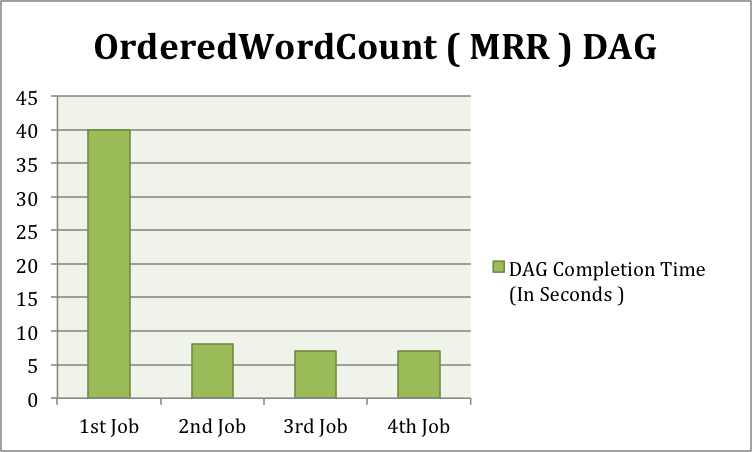
\includegraphics[width=0.48\textwidth]{sessions-tez2}
        \caption{tez01}
        \label{fig18}
\end{figure}

As you can see, even though this is just a simulation test running on a
\emph{very small data} set, leveraging containers across DAGs has a huge
performance benefit.

\bibliographystyle{IEEEtran}
\bibliography{References}

\section*{Appendix}



\end{document}
